%!TEX encoding = UTF-8 Unicode

\section{Introduction}

%\epigraph{If language was given to men to conceal their thoughts, then gesture's purpose was to disclose them.}{John Napier, \emph{Hands}}

Robotics is progressing fast, with a steady and systematic shift from the industrial domain to domestic, public and leisure environments. Application areas that are particularly relevant and being researched by the scientific community include: robots for people's health and active aging, mobility, advanced manufacturing~(Industry~4.0). In short, all domains that require direct and effective \hri and communication.

However, robots have not reached the level of performance that would enable them to work with humans in routine activities in a flexible and adaptive way, for example in the presence of sensor noise, or unexpected events not previously seen during the training or learning phase. One of the reasons to explain this performance gap between \hh{} teamwork and a \hr{} teamwork is in the collaboration aspect, \ie, whether the members of a team understand one another. Humans have the ability of working successfully in groups. They can agree on common goals~(\eg, through verbal and non-verbal communication), work towards the execution of these goals in a coordinated way, and understand each other's physical actions~(\eg, body gestures) towards the realization of the final target. Human team coordination and mutual understanding is effective~\cite{ramnani:2004:natureneuro} because of~(i) the capacity to \emph{adapt} to unforeseen events in the environment, and re-plan one's actions in real time if necessary, and~(ii) a common motor repertoire and action model, which permits us to understand a partner's physical actions and manifested intentions as if they were our own.

In neuroscience research, visuomotor neurons~(\ie, neurons that are activated by visual stimuli) have been a subject of ample study~\cite{rizzolatti:2001:nrn}. Mirror neurons are one class of such neurons that responds to action and object interaction, both when the agent acts and when it observes the same action performed by others, hence the name ``mirror''.

\begin{figure}
  \centering
  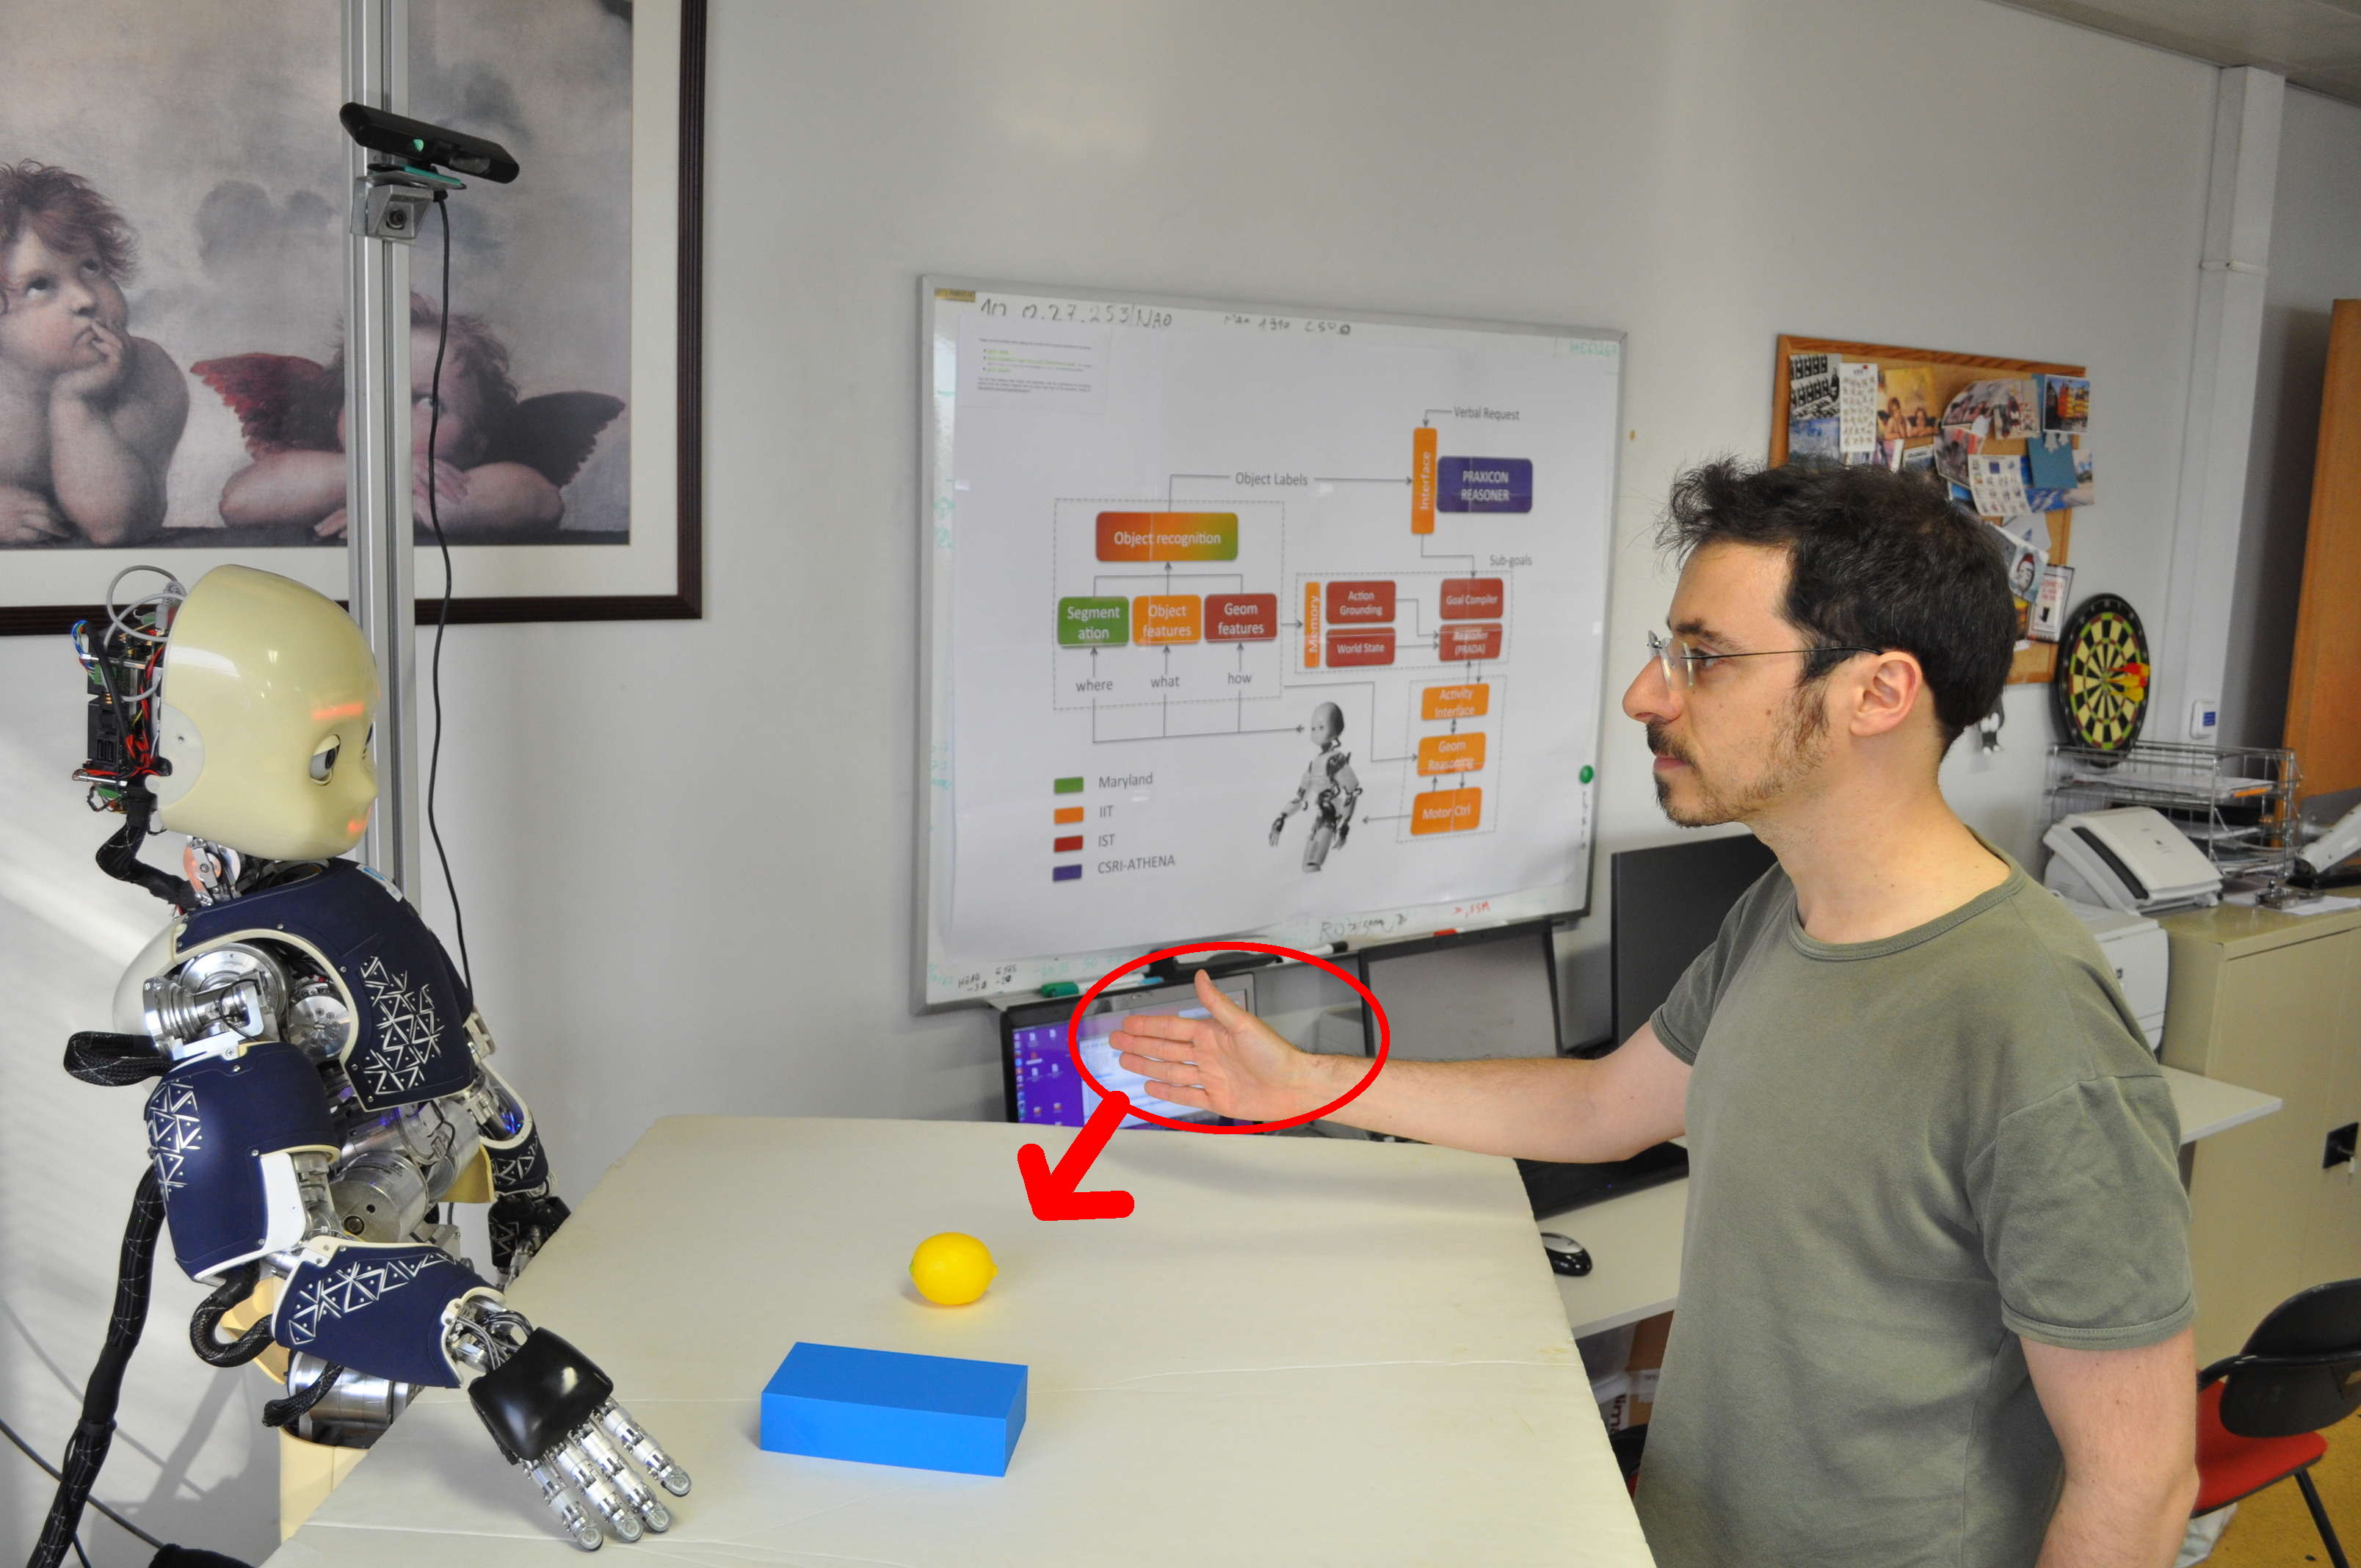
\includegraphics[width=0.9\columnwidth]{human_tap}
  \caption{Setup.}
  \label{fig:human_tap}
\end{figure}

This work is framed within the theory of mirror neurons, and contributes towards testing it on humanoid and cognitive robots. We show that a robot can first acquire knowledge by sensing and self-exploring its surrounding environment~(\eg, by interacting with available objects and building up an affordance representation of the interactions and their outcomes) and, as a result, the robot is capable of generalizing its acquired knowledge while observing another agent~(\eg, a human person) who performs similar physical actions to the ones executed during prior robot training.
